% Options for packages loaded elsewhere
\PassOptionsToPackage{unicode}{hyperref}
\PassOptionsToPackage{hyphens}{url}
%
\documentclass[
  english,
  man,floatsintext]{apa6}
\usepackage{lmodern}
\usepackage{amssymb,amsmath}
\usepackage{ifxetex,ifluatex}
\ifnum 0\ifxetex 1\fi\ifluatex 1\fi=0 % if pdftex
  \usepackage[T1]{fontenc}
  \usepackage[utf8]{inputenc}
  \usepackage{textcomp} % provide euro and other symbols
\else % if luatex or xetex
  \usepackage{unicode-math}
  \defaultfontfeatures{Scale=MatchLowercase}
  \defaultfontfeatures[\rmfamily]{Ligatures=TeX,Scale=1}
\fi
% Use upquote if available, for straight quotes in verbatim environments
\IfFileExists{upquote.sty}{\usepackage{upquote}}{}
\IfFileExists{microtype.sty}{% use microtype if available
  \usepackage[]{microtype}
  \UseMicrotypeSet[protrusion]{basicmath} % disable protrusion for tt fonts
}{}
\makeatletter
\@ifundefined{KOMAClassName}{% if non-KOMA class
  \IfFileExists{parskip.sty}{%
    \usepackage{parskip}
  }{% else
    \setlength{\parindent}{0pt}
    \setlength{\parskip}{6pt plus 2pt minus 1pt}}
}{% if KOMA class
  \KOMAoptions{parskip=half}}
\makeatother
\usepackage{xcolor}
\IfFileExists{xurl.sty}{\usepackage{xurl}}{} % add URL line breaks if available
\IfFileExists{bookmark.sty}{\usepackage{bookmark}}{\usepackage{hyperref}}
\hypersetup{
  pdftitle={The relation between search asymmetry and metacognitive asymmetry},
  pdflang={en-EN},
  pdfkeywords={keywords},
  hidelinks,
  pdfcreator={LaTeX via pandoc}}
\urlstyle{same} % disable monospaced font for URLs
\usepackage{graphicx,grffile}
\makeatletter
\def\maxwidth{\ifdim\Gin@nat@width>\linewidth\linewidth\else\Gin@nat@width\fi}
\def\maxheight{\ifdim\Gin@nat@height>\textheight\textheight\else\Gin@nat@height\fi}
\makeatother
% Scale images if necessary, so that they will not overflow the page
% margins by default, and it is still possible to overwrite the defaults
% using explicit options in \includegraphics[width, height, ...]{}
\setkeys{Gin}{width=\maxwidth,height=\maxheight,keepaspectratio}
% Set default figure placement to htbp
\makeatletter
\def\fps@figure{htbp}
\makeatother
\setlength{\emergencystretch}{3em} % prevent overfull lines
\providecommand{\tightlist}{%
  \setlength{\itemsep}{0pt}\setlength{\parskip}{0pt}}
\setcounter{secnumdepth}{-\maxdimen} % remove section numbering
% Make \paragraph and \subparagraph free-standing
\ifx\paragraph\undefined\else
  \let\oldparagraph\paragraph
  \renewcommand{\paragraph}[1]{\oldparagraph{#1}\mbox{}}
\fi
\ifx\subparagraph\undefined\else
  \let\oldsubparagraph\subparagraph
  \renewcommand{\subparagraph}[1]{\oldsubparagraph{#1}\mbox{}}
\fi
% Manuscript styling
\usepackage{upgreek}
\captionsetup{font=singlespacing,justification=justified}

% Table formatting
\usepackage{longtable}
\usepackage{lscape}
% \usepackage[counterclockwise]{rotating}   % Landscape page setup for large tables
\usepackage{multirow}		% Table styling
\usepackage{tabularx}		% Control Column width
\usepackage[flushleft]{threeparttable}	% Allows for three part tables with a specified notes section
\usepackage{threeparttablex}            % Lets threeparttable work with longtable

% Create new environments so endfloat can handle them
% \newenvironment{ltable}
%   {\begin{landscape}\begin{center}\begin{threeparttable}}
%   {\end{threeparttable}\end{center}\end{landscape}}
\newenvironment{lltable}{\begin{landscape}\begin{center}\begin{ThreePartTable}}{\end{ThreePartTable}\end{center}\end{landscape}}

% Enables adjusting longtable caption width to table width
% Solution found at http://golatex.de/longtable-mit-caption-so-breit-wie-die-tabelle-t15767.html
\makeatletter
\newcommand\LastLTentrywidth{1em}
\newlength\longtablewidth
\setlength{\longtablewidth}{1in}
\newcommand{\getlongtablewidth}{\begingroup \ifcsname LT@\roman{LT@tables}\endcsname \global\longtablewidth=0pt \renewcommand{\LT@entry}[2]{\global\advance\longtablewidth by ##2\relax\gdef\LastLTentrywidth{##2}}\@nameuse{LT@\roman{LT@tables}} \fi \endgroup}

% \setlength{\parindent}{0.5in}
% \setlength{\parskip}{0pt plus 0pt minus 0pt}

% \usepackage{etoolbox}
\makeatletter
\patchcmd{\HyOrg@maketitle}
  {\section{\normalfont\normalsize\abstractname}}
  {\section*{\normalfont\normalsize\abstractname}}
  {}{\typeout{Failed to patch abstract.}}
\makeatother
\shorttitle{asymmetry}
\author{Matan Mazor\textsuperscript{1}\ \& Stephen M. Fleming\textsuperscript{1,2,3}}
\affiliation{
\vspace{0.5cm}
\textsuperscript{1} Wellcome Centre for Human Neuroimaging, UCL\\\textsuperscript{2} Max Planck UCL Centre for Computational Psychiatry and Ageing Research\\\textsuperscript{3} Department of Experimental Psychology, UCL}
\authornote{

Correspondence concerning this article should be addressed to Matan Mazor, 12 Queen Square, London WC1N 3BG. E-mail: mtnmzor@gmail.com}
\keywords{keywords\newline\indent Word count: 2214}
\usepackage{lineno}

\linenumbers
\usepackage{csquotes}
\ifxetex
  % Load polyglossia as late as possible: uses bidi with RTL langages (e.g. Hebrew, Arabic)
  \usepackage{polyglossia}
  \setmainlanguage[]{english}
\else
  \usepackage[shorthands=off,main=english]{babel}
\fi

\title{The relation between search asymmetry and metacognitive asymmetry}

\date{}

\abstract{
Subjective confidence judgments are more aligned with objective performance following decisions about the presence, rather than the absence, of a stimulus or a memory. Here we ask whether this metacognitive asymmetry reflects a conceptual difference between the higher-level representation of presence and absence, or alternatively result from distributional properties of these two types of representations. By leveraging the visual search asymmetry phenomenon, we ask whether a metacognitive asymmetry exists for discrimination decisions about stimulus pairs that differ by the presence of a stimulus feature.
}

\begin{document}
\maketitle

\hypertarget{introduction}{%
\section{Introduction}\label{introduction}}

In detection (\emph{Was there a stimulus present or not?}), subjective confidence ratings following \enquote{target absent} judgments are commonly lower, and less correlated with objective accuracy, than following \enquote{target present} judgments (Kanai, Walsh, \& Tseng, 2010; Kellij, Fahrenfort, Lau, Peters, \& Odegaard, 2018; Mazor, Friston, \& Fleming, 2020; Meuwese, Loon, Lamme, \& Fahrenfort, 2014). This \emph{metacognitive asymmetry} is present not only for detection tasks, but also for recognition memory (Higham, Perfect, \& Bruno, 2009) and lexicality judgments (Fleming \& Dolan, 2010) -- both can be described as detection among items in an internal representation space (memory storage, orthographic lexicon). According to one interpretation, this metacognitive asymmetry reflects a qualitative difference between the metacognitive representations of decisions that are driven by the presence or the absence of evidence (Meuwese et al., 2014). One variant of this interpretation posits that the metacognitive evaluation of negative judgments is more computationally demanding because instead of relying on evidence for absence, it relies on the counterfactual likelihood of evidence for presence (contrast ``I saw it was not there'' with ``If it was there I would not have missed it''; Mazor et al., 2020). In contrast, this asymmetry can also be interpreted as reflecting an asymmetry in the perceptual and cognitive uncertainties that are associated with the representations of presence and absence. For example, Kellij et al. (2018) successfully replicated the metacognitive asymmetry effect in a simple Signal Detection Theory (SDT) model with higher signal variance. Their model did not have to posit any asymmetry in higher-order processes in order to fit the empirical data.

The higher- and first-order interpretations of the metacognitive asymmetry resemble the controversy about the interpretation of another behavioural asymmetry. Searching for one \emph{Q} among 10 \emph{O}'s is easier than searching for one \emph{O} among 10 \emph{Q}s. This long known \emph{search asymmetry} (Treisman \& Souther, 1985) is present not only for other shapes (\emph{C}-in-\emph{O} search is easier than the inverse \emph{O}-in-\emph{C} search; Treisman \& Souther, 1985; Takeda \& Yagi, 2000; Treisman \& Gormican, 1988), but also for certain color pairs (magenta-in-red search is easier than red-in-magenta search; Treisman \& Gormican, 1988), curvature (curved-in-straight search is easier than straight-in-curved search; Treisman \& Gormican, 1988), and higher-level stimulus attributes such as spatial orientation (Von Grünau \& Dubé, 1994) and familiarity (Frith, 1974; Wang, Cavanagh, \& Green, 1994). Furthermore, search asymmetry is present early in development (as early as 3 months; Adler \& Gallego, 2014; Colombo, Ryther, Frick, \& Gifford, 1995), and in other phylogenetically remote species (for example, pigeons; Pearce \& George, 2003).

Over the years researchers proposed different theoretical accounts for this phenomenon. Treisman and Souther (1985) proposed that visual search is more efficient when searching for the presence, rather than the absence, of a stimulus feature. According to this account, the letter \emph{Q} is marked by an additional feature (a diagonal line) compared to the baseline \emph{O}. Similarly, blue is present in magenta but absent in red. Treisman and Gormican (1988) then used search-asymmetry as a litmus test for what counts as presence and what counts as absence in early vision. For example, the fact that \emph{C}-in-\emph{O} search is easier than \emph{O}-in-\emph{C} search was used as evidence for that \enquote{free ends}, rather than shape-closeness, are positively encoded in vision. Contextual effects have led Treisman and Gormican (1988) to further propose that search asymmetry can in some cases originate from a deviation from a default state (also termed null, prototypical, or standard state). This standard state is affected by prior knowledge and available context, for example searching for a tilted line among vertical distractors is easier than the inverse search, but this effect reverses when the search array is displayed inside a tilted frame (Treisman \& Gormican, 1988). The contents of the default state are partly hard-coded into the wiring of the system (like in the case of color) and partly affected by expectations that are sensitive to context and prior experience (like in the cases of viewing direction or familiarity with letters; Von Grünau \& Dubé, 1994; Wang et al., 1994).

\begin{figure}
\centering
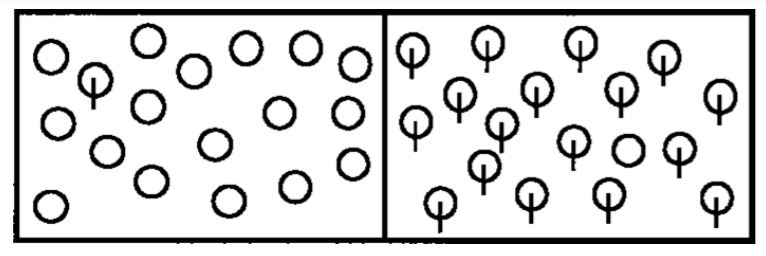
\includegraphics{figures/wolfeexample.png}
\caption{It is easier to find the circle with the vertical line among plain circles (left panel) than vice versa. Adapted from Wolfe (2001)}
\end{figure}

Treisman and Gormican (1988) interpreted search asymmetries as revealing a categorical difference between pre-attentive parallel search and attention-guided serial search. According to their account, parallel search is not available when searching for a target that is marked by the absence, or the lesser quantity, of a feature, and when searching for a prototypical stimulus among deviant distractors. This is in line with the proposal that the representation of absence is cognitively demanding and is not available without the active engagement of attention. In contrast, probabilistic parallel models of visual search, inspired by Signal Detection Theory, frame search asymmetry effects not as marking a categorical difference between serial and parallel search, but as reflecting the effect of stimulus uncertainty on the noisiness of the search process which is always parallel (Dosher, Han, \& Lu, 2004; Vincent, 2011). Vincent (2011) demonstrated that differences in search efficiency can be accounted for by the \emph{sigma ratio}: the relative difference in internal uncertainty associated with the two stimulus categories. He found support for his sigma-ratio account in the slope of standardized ROC curves, extracted from subjective confidence estimates in a vertical/tilted visual search task. Similarly, reverse correlation analysis revealed higher variability in the internal representation of \emph{Q}, compared to \emph{O}, stimuli (Saiki, 2008). It is important to note here that the parallel/serial account also predicts sensitivity of search slope to variability in internal representations. For example, Treisman and Gormican (1988) relied on Weber's law to show that searching for a target that induces increased activity compared to distractors is more efficient than searching for a target that induces weaker activity, due to differences in the underlying noise level.

In this study, we will compare search- and metacognitive asymmetries across several stimulus features, in order to ask whether the two effects reflect the behavioural signature of identical, partly-overlapping, or completely distinct mechanisms. We will test the hypothesis that the two asymmetries result from differences in the shape of the underlying signal distributions for the two stimulus categories. \emph{MM: I am not sure how to test this hypothesis}

More specifically, this study is set to test the following hypotheses:

\begin{enumerate}
\def\labelenumi{\arabic{enumi}.}
\tightlist
\item
  \textbf{Hypothesis 1}: Metacognitive asymmetry, measured as the area between the two response conditional ROC curves, follows the same direction as search asymmetry.
\end{enumerate}

This hypothesis will be tested for the following stimulus features for which search asymmetry has been demonstrated: addition of a stimulus part, open ends, color, curvature, orientation and familiarity. We will test Hypothesis 1 separately for each stimulus feature, by replicating the original search asymmetry (for example, Q-in-O search is more efficient that O-in-Q search) and testing the null hypothesis that metacognitive sensitivity (measured as the area under the response conditional ROC curve) for the efficient target (e.g., \emph{Q}) is equal to or lower than metacognitive sensitivity for the inefficient target (e.g., for the case of \emph{Q}/\emph{O}, \(H_o=auROC_{Q}\leq auROC_O\)).

\begin{enumerate}
\def\labelenumi{\arabic{enumi}.}
\setcounter{enumi}{1}
\tightlist
\item
  \textbf{Hypothesis 2}: Individual differences in the direction and magnitude of search asymmetry positively covary with individual differences in the direction and magnitude of metacognitive asymmetry. This hypothesis will be tested globally for the 6 experiments by fitting a mixed-effects linear model using the \texttt{brms} package (Bürkner \& Buerkner, 2016).
\end{enumerate}

\hypertarget{methods}{%
\section{Methods}\label{methods}}

We report how we determined our sample size, all data exclusions (if any), all manipulations, and all measures in the study.

\hypertarget{participants}{%
\subsection{Participants}\label{participants}}

For each of the six experiments, we will collect data until we reach 200 included participants (after applying our pre-registered exclusion criteria). With 200 participants, we will have a statistical power of 95\% to detect effects of size 0.23, which is about half the effect size we observed for metacognitive asymmetry and less than fifth the effect size we observed for search slopes in our pilot sample.

Multi-level MCMC simulations, assuming an average correlation of 0.29 across the six tasks between search and metacognitive asymmetries, indicated a statistical power of 97\% to reject the null hypothesis for Hypothesis 2.

\hypertarget{material}{%
\subsection{Material}\label{material}}

\hypertarget{procedure}{%
\subsection{Procedure}\label{procedure}}

Experiments will be identical, except for the identity of the target and distractor stimuli. In what follows we will describe the procedure for the stimulus pair \enquote{\emph{Q}} and \enquote{\emph{O}}. See Experiment here: \url{https://visual-search-c-o.glitch.me}

The Experiment will comprise three parts (\enquote{challenges}) presented in pseudorandomized order.

\begin{enumerate}
\def\labelenumi{\arabic{enumi}.}
\item
  The first part will comprise 32 visual search trials. In these trials participants will search for one \enquote{\emph{Q}} in an array of 1, 2, 4 or 8 \enquote{\emph{O}} distractors. The target stimulus will be present in half of the trials, and absent in the other half. Participants will be instructed to use their keyboard to indicate whether the target was present (press J) or absent (press F) as quickly and accurately as possible. Each trial will start with an instruction screen, indicating the search target (500-1000 ms), followed by the presentation of the search array. The search array will remain visible until a response is recorded. Feedback about accuracy will be delivered. To motivate accurate responses, the feedback screen will remain for 1000 ms following correct responses and for 4000 ms following incorrect responses. The visual search block will start with four practice trials of distractor set-size 4 that will not be included in the final analysis. The actual block of 32 trials will start once all four practice trials are answered correctly, otherwise additional practice trials will be delivered.
\item
  The second part will be identical to the first part, except for the identity of the target stimulus. Here \enquote{\emph{O}} will server as target and \enquote{\emph{Q}} as distractor.
\item
  In the third part, participants will make discrimination judgments between masked \emph{Q} and \emph{O} stimuli, and rate their subjective decision confidence on a continuous scale. After a fixation cross (500 ms), the target stimulus will be presented in the center of the screen for 50 ms, followed by a mask (100 ms). Stimulus onset asynchrony will be calibrated online in a 1-up-2-down procedure (Levitt, 1971), with a multiplicative step factor of 0.9, and starting from 30 milliseconds. Participants will then use their keyboard to make a discrimination judgment. Following their response, subjective confidence ratings will be given on an analog scale by controlling the size of a colored circle with the computer mouse. High confidence will be mapped to a big, blue circle, and low confidence to a small, red circle. The confidence rating phase will terminate once participants click their mouse, but not before 2000 ms. No feedback will be delivered about accuracy.
\end{enumerate}

\begin{figure}
\centering
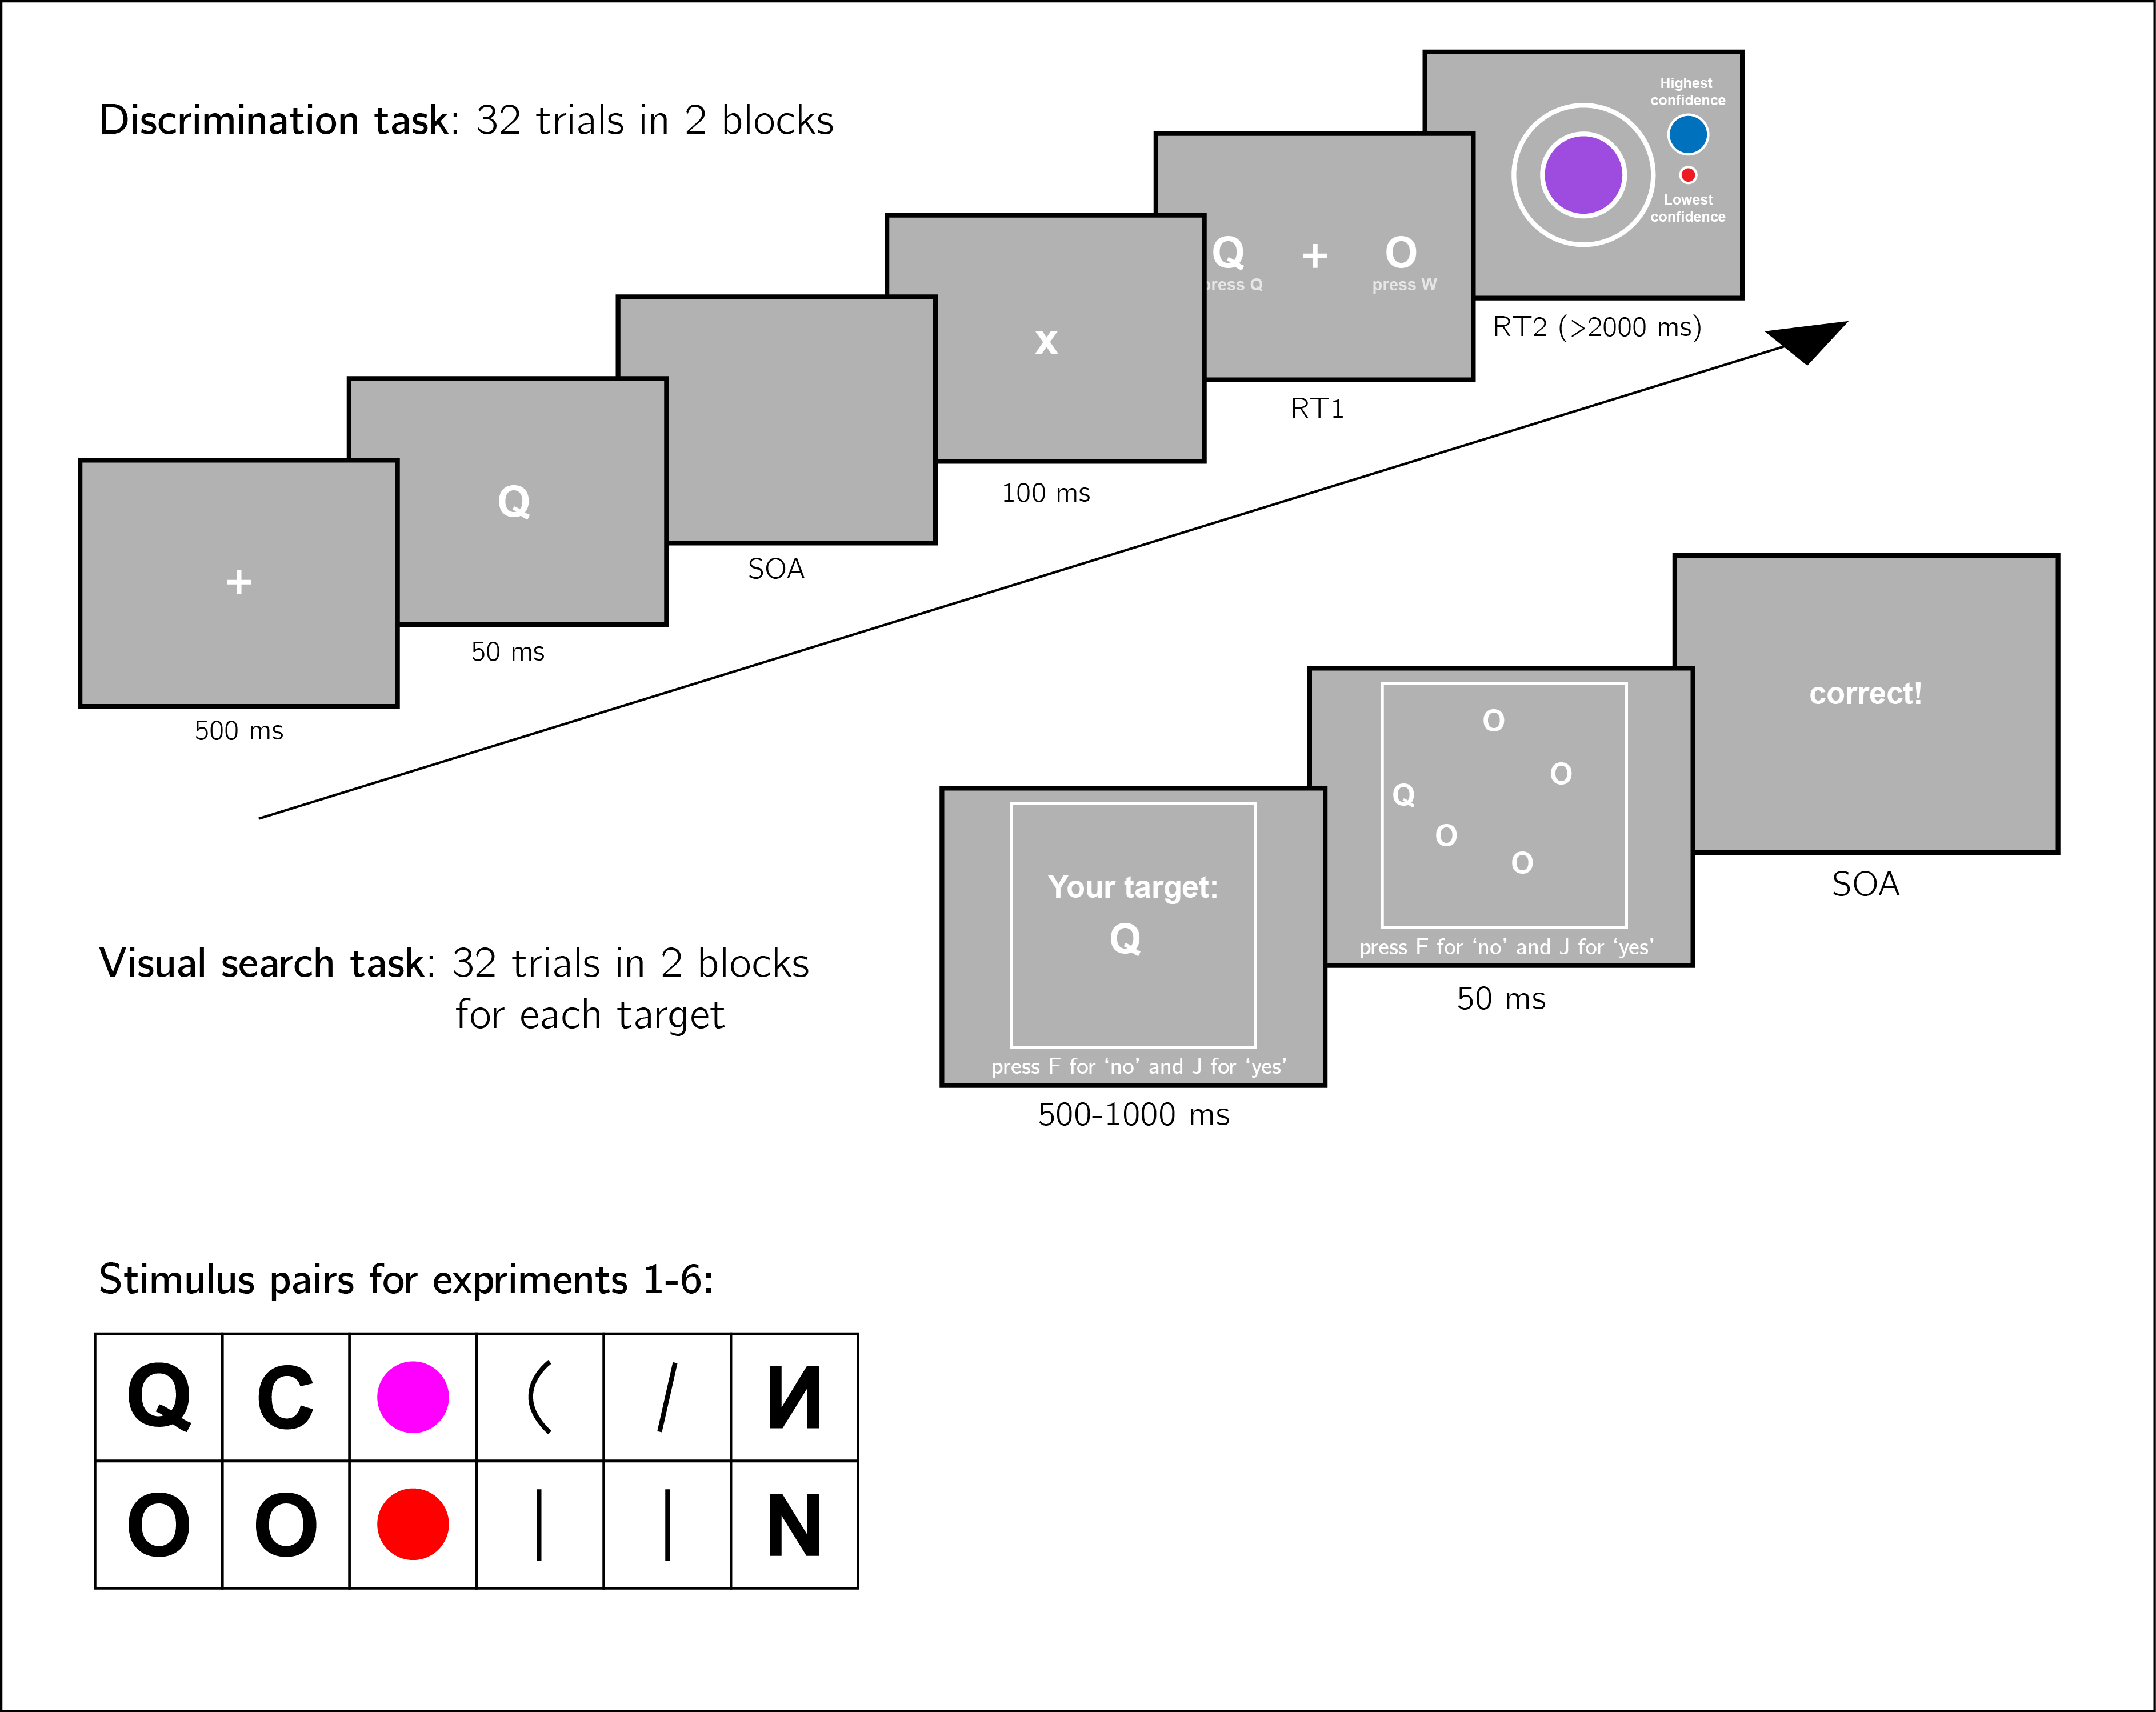
\includegraphics{figures/trial_structure.png}
\caption{Experiment structure. Three experimental parts will be delivered in pseudorandomized order: a discrimination task with subjective confidence ratings, and two visual search tasks with different distractor/target assignments. Asymmetry effects will be tested for six stimulus features in six separate experiments.}
\end{figure}

We will test the following stimulus features in separate experiments:

\begin{enumerate}
\def\labelenumi{\arabic{enumi}.}
\tightlist
\item
  \textbf{Addition of a stimulus part}. \emph{Q} and \emph{O} will be used as stimuli (Treisman \& Souther, 1985).
\item
  \textbf{Open ends}. \emph{C} and \emph{O} will be used as stimuli (Takeda \& Yagi, 2000; Treisman \& Gormican, 1988; Treisman \& Souther, 1985).
\item
  \textbf{Color}. Red and magenta dots will be used as stimuli (Treisman \& Gormican, 1988).
\item
  \textbf{Curvature}. Straight and curved lines will be used as stimuli (Treisman \& Gormican, 1988).
\item
  \textbf{Orientation}. Vertical and tilted lines will be used as stimuli (Treisman \& Gormican, 1988).
\item
  \textbf{Familiarity}. Reversed and normal \emph{N} will be used as stimuli (Frith, 1974).
\end{enumerate}

\hypertarget{data-analysis}{%
\subsection{Data analysis}\label{data-analysis}}

We will use R (Version 3.6.0; R Core Team, 2019) and the R-packages \emph{brms} (Version 2.13.0; Bürkner, 2018), \emph{broom} (Version 0.5.6; Robinson \& Hayes, 2020), \emph{cowplot} (Version 1.0.0; Wilke, 2019), \emph{dplyr} (Version 1.0.0; Wickham et al., 2020), \emph{ggplot2} (Version 3.3.1; Wickham, 2016), \emph{papaja} (Version 0.1.0.9942; Aust \& Barth, 2020), and \emph{tidyr} (Version 1.1.0; Wickham \& Henry, 2020) for all our analyses.

\hypertarget{rejection-criteria}{%
\subsubsection{Rejection criteria}\label{rejection-criteria}}

Participants will be excluded for performing below 70\% accuracy in one or two of the search tasks, for performing below 60\% accuracy in the discrimination task, for having extremely fast or slow reaction times in one or more of the tasks (below 250 milliseconds or above 5 seconds in more than 25\% of the trials), and for failing the comprehension check. For the response-conditional ROC analysis, only participants that committed at least one error of each error type (for example, mistaking a \emph{Q} of \emph{O} and mistaking an \emph{O} for \emph{Q}), will be included.

Trials with response-time below 250 milliseconds or above 5 seconds will be excluded.

Only correct visual search trials will be analyzed.

\hypertarget{dependent-variables-and-analysis-plan}{%
\subsubsection{Dependent variables and analysis plan}\label{dependent-variables-and-analysis-plan}}

The following measures will be extracted for each participant:
1. The difference between the area under the response-conditional type-2 ROC curves for the two responses {[}e.g., \enquote{\emph{Q}} and \enquote{\emph{O}}{]}: \(\Delta_m\). The area between the two curves is a measure of metacognitive asymmetry. This difference will be used to test Hypothesis 1.
2. The difference between search slopes for the two visual search tasks (defined as \(\beta_1\) in the linear regression model \(RT=\beta_0+\beta_1set\_size\), collapsed across both \enquote{yes} and \enquote{no} responses): \(\Delta_s\). The difference between the curves is a measure of search asymmetry. This difference will be used to test Hypothesis 1.
3. The relative difference between the area under the response-conditional type-2 ROC curves for the two responses (\(\Delta^{rel}_m\)) will be defined as the area between the two curves, divided by the sum of the areas under the two curves. This relative difference will be used in the hierarchical model to test Hypothesis 2.
4. The relative difference between search slopes for the two visual search tasks (\(\Delta^{rel}_s\)) will be defined as the difference between the two search slopes, divided by their sum. This relative difference will be used in the hierarchical model to test Hypothesis 2.

For each of the six experiments, Hypothesis 1 (metacognitive asymmetry follows the same direction as search asymmetry) will be tested using a one tailed t-test at the group level with \(\alpha=0.05\). In case of a null result, a two one-sided test (TOST procedure; Schuirmann, 1987) will be adopted to test the null hypothesis that \(|\Delta_m|\) is higher than the smallest effect size of interest (0.05 in auROC units, ranging from 0 to 1), or that \(|\Delta_s|\) is higher than the smallest effect size of interest (1 millisecond/item).

Hypothesis 2 (search and metacognitive asymmetries covary) will be tested globally for the 6 experiments by fitting a mixed-effects linear model using the \texttt{brms} package (Bürkner \& Buerkner, 2016). The following mixed-effects linear model will be fitted to the data: \(\Delta^{rel}_s \sim 1+\Delta^{rel}_m+(1+\Delta^{rel}_m | exp)\) where \(exp\) denoted the specific experiment in which the subject participated. The population-level coefficient for \(\Delta^{rel}_s\) will be compared against 0. We will conclude that the two effects are correlated at the population level if the lower bound of the 95\% credible interval for this coefficient will by higher than 0.05. We will conclude that the correlation falls within our Region of Practical Equivalence (Kruschke, 2013) if the entire credible interval will fall within the region \([-0.05, 0.05]\).

\newpage

\hypertarget{references}{%
\section{References}\label{references}}

\begingroup
\setlength{\parindent}{-0.5in}
\setlength{\leftskip}{0.5in}

\hypertarget{refs}{}
\leavevmode\hypertarget{ref-adler2014search}{}%
Adler, S. A., \& Gallego, P. (2014). Search asymmetry and eye movements in infants and adults. \emph{Attention, Perception, \& Psychophysics}, \emph{76}(6), 1590--1608.

\leavevmode\hypertarget{ref-R-papaja}{}%
Aust, F., \& Barth, M. (2020). \emph{papaja: Create APA manuscripts with R Markdown}. Retrieved from \url{https://github.com/crsh/papaja}

\leavevmode\hypertarget{ref-R-brms_b}{}%
Bürkner, P.-C. (2018). Advanced Bayesian multilevel modeling with the R package brms. \emph{The R Journal}, \emph{10}(1), 395--411. \url{https://doi.org/10.32614/RJ-2018-017}

\leavevmode\hypertarget{ref-burkner2016package}{}%
Bürkner, P.-C., \& Buerkner, M. P.-C. (2016). Package ``brms''.

\leavevmode\hypertarget{ref-colombo1995visual}{}%
Colombo, J., Ryther, J. S., Frick, J. E., \& Gifford, J. J. (1995). Visual pop-out in infants: Evidence for preattentive search in 3-and 4-month-olds. \emph{Psychonomic Bulletin \& Review}, \emph{2}(2), 266--268.

\leavevmode\hypertarget{ref-dosher2004parallel}{}%
Dosher, B. A., Han, S., \& Lu, Z.-L. (2004). Parallel processing in visual search asymmetry. \emph{Journal of Experimental Psychology: Human Perception and Performance}, \emph{30}(1), 3.

\leavevmode\hypertarget{ref-fleming2010effects}{}%
Fleming, S. M., \& Dolan, R. J. (2010). Effects of loss aversion on post-decision wagering: Implications for measures of awareness. \emph{Consciousness and Cognition}, \emph{19}(1), 352--363.

\leavevmode\hypertarget{ref-frith1974acurious}{}%
Frith, U. (1974). Acurious effect with reversed letters explained by a theory of schema. \emph{Perception \& Psychophysics}, \emph{16}(1), 113--116.

\leavevmode\hypertarget{ref-higham2009investigating}{}%
Higham, P. A., Perfect, T. J., \& Bruno, D. (2009). Investigating strength and frequency effects in recognition memory using type-2 signal detection theory. \emph{Journal of Experimental Psychology: Learning, Memory, and Cognition}, \emph{35}(1), 57.

\leavevmode\hypertarget{ref-kanai2010subjective}{}%
Kanai, R., Walsh, V., \& Tseng, C.-h. (2010). Subjective discriminability of invisibility: A framework for distinguishing perceptual and attentional failures of awareness. \emph{Consciousness and Cognition}, \emph{19}(4), 1045--1057.

\leavevmode\hypertarget{ref-kellij2018foundations}{}%
Kellij, S., Fahrenfort, J., Lau, H., Peters, M. A., \& Odegaard, B. (2018). The foundations of introspective access: How the relative precision of target encoding influences metacognitive performance.

\leavevmode\hypertarget{ref-kruschke2013much}{}%
Kruschke, J. (2013). How much of a bayesian posterior distribution falls inside a region of practical equivalence (rope). \emph{Doing Bayesian Data Analysis Web Blog Post}.

\leavevmode\hypertarget{ref-levitt1971transformed}{}%
Levitt, H. (1971). Transformed up-down methods in psychoacoustics. \emph{The Journal of the Acoustical Society of America}, \emph{49}(2B), 467--477.

\leavevmode\hypertarget{ref-mazor2020distinct}{}%
Mazor, M., Friston, K. J., \& Fleming, S. M. (2020). Distinct neural contributions to metacognition for detecting, but not discriminating visual stimuli. \emph{Elife}, \emph{9}, e53900.

\leavevmode\hypertarget{ref-meuwese2014subjective}{}%
Meuwese, J. D., Loon, A. M. van, Lamme, V. A., \& Fahrenfort, J. J. (2014). The subjective experience of object recognition: Comparing metacognition for object detection and object categorization. \emph{Attention, Perception, \& Psychophysics}, \emph{76}(4), 1057--1068.

\leavevmode\hypertarget{ref-pearce2003visual}{}%
Pearce, J. M., \& George, D. N. (2003). Visual search asymmetry in pigeons. \emph{Journal of Experimental Psychology: Animal Behavior Processes}, \emph{29}(2), 118.

\leavevmode\hypertarget{ref-R-base}{}%
R Core Team. (2019). \emph{R: A language and environment for statistical computing}. Vienna, Austria: R Foundation for Statistical Computing. Retrieved from \url{https://www.R-project.org/}

\leavevmode\hypertarget{ref-R-broom}{}%
Robinson, D., \& Hayes, A. (2020). \emph{Broom: Convert statistical analysis objects into tidy tibbles}. Retrieved from \url{https://CRAN.R-project.org/package=broom}

\leavevmode\hypertarget{ref-saiki2008stimulus}{}%
Saiki, J. (2008). Stimulus-driven mechanisms underlying visual search asymmetry revealed by classification image analyses. \emph{Journal of Vision}, \emph{8}(4), 30--30.

\leavevmode\hypertarget{ref-schuirmann1987comparison}{}%
Schuirmann, D. J. (1987). A comparison of the two one-sided tests procedure and the power approach for assessing the equivalence of average bioavailability. \emph{Journal of Pharmacokinetics and Biopharmaceutics}, \emph{15}(6), 657--680.

\leavevmode\hypertarget{ref-takeda2000inhibitory}{}%
Takeda, Y., \& Yagi, A. (2000). Inhibitory tagging in visual search can be found if search stimuli remain visible. \emph{Perception \& Psychophysics}, \emph{62}(5), 927--934.

\leavevmode\hypertarget{ref-treisman1988feature}{}%
Treisman, A., \& Gormican, S. (1988). Feature analysis in early vision: Evidence from search asymmetries. \emph{Psychological Review}, \emph{95}(1), 15.

\leavevmode\hypertarget{ref-treisman1985search}{}%
Treisman, A., \& Souther, J. (1985). Search asymmetry: A diagnostic for preattentive processing of separable features. \emph{Journal of Experimental Psychology: General}, \emph{114}(3), 285.

\leavevmode\hypertarget{ref-vincent2011search}{}%
Vincent, B. T. (2011). Search asymmetries: Parallel processing of uncertain sensory information. \emph{Vision Research}, \emph{51}(15), 1741--1750.

\leavevmode\hypertarget{ref-von1994visual}{}%
Von Grünau, M., \& Dubé, S. (1994). Visual search asymmetry for viewing direction. \emph{Perception \& Psychophysics}, \emph{56}(2), 211--220.

\leavevmode\hypertarget{ref-wang1994familiarity}{}%
Wang, Q., Cavanagh, P., \& Green, M. (1994). Familiarity and pop-out in visual search. \emph{Perception \& Psychophysics}, \emph{56}(5), 495--500.

\leavevmode\hypertarget{ref-R-ggplot2}{}%
Wickham, H. (2016). \emph{Ggplot2: Elegant graphics for data analysis}. Springer-Verlag New York. Retrieved from \url{https://ggplot2.tidyverse.org}

\leavevmode\hypertarget{ref-R-dplyr}{}%
Wickham, H., François, R., Henry, L., \& Müller, K. (2020). \emph{Dplyr: A grammar of data manipulation}. Retrieved from \url{https://CRAN.R-project.org/package=dplyr}

\leavevmode\hypertarget{ref-R-tidyr}{}%
Wickham, H., \& Henry, L. (2020). \emph{Tidyr: Tidy messy data}. Retrieved from \url{https://CRAN.R-project.org/package=tidyr}

\leavevmode\hypertarget{ref-R-cowplot}{}%
Wilke, C. O. (2019). \emph{Cowplot: Streamlined plot theme and plot annotations for 'ggplot2'}. Retrieved from \url{https://CRAN.R-project.org/package=cowplot}

\leavevmode\hypertarget{ref-wolfe2001asymmetries}{}%
Wolfe, J. M. (2001). Asymmetries in visual search: An introduction. \emph{Perception \& Psychophysics}, \emph{63}(3), 381--389.

\endgroup

\newpage

\hypertarget{supplementary-information}{%
\section{Supplementary information}\label{supplementary-information}}

\hypertarget{pilot-data-and-analysis}{%
\section{Pilot data and analysis}\label{pilot-data-and-analysis}}

30 participants were recruited from Prolific for our pilot experiment. We followed the procedure described in the Methods section, using \emph{Q} and \emph{O} as our stimuli. The experiment took about 10 minutes to complete. Subjects were paid £1.25 for their participation.

Mean accuracy was 0.80 in the discrimination task, 0.96 in the Q-in-O search task, and 0.95 in the O-in-Q search task. We excluded participants for performing below 70\% accuracy in one or two of the search tasks, for performing below 60\% accuracy in the discrimination task, for having extremely fast or slow reaction times in one or more of the tasks (below 250 milliseconds or above 5 seconds in more than 25\% of the trials), and for failing the comprehension check. Overall we excluded 0 participants, leaving 30 participants for the main analysis.

\hypertarget{visual-search-task-search-asymmetry}{%
\subsection{Visual search task: search asymmetry}\label{visual-search-task-search-asymmetry}}

Search time analysis was performed on correct trials with reaction time between 250 and 5000 milliseconds. Search slopes for the response time/set size function were extracted for each participant, task and response, and then subjected to a two-way analysis of variance. As expected, we observed significant effects for target identity (mean search slope for \emph{Q-in-O} search: 18.93 ms/item; mean search slope for \emph{O-in-Q} search: 54.89 ms/item; \(F(1, 116) = 44.39\), \(\mathit{MSE} = 873.80\), \(p < .001\)) and response (mean search slope for target absent responses: 48.04; mean search slope for target present responses: 25.78; \(F(1, 116) = 17.01\), \(\mathit{MSE} = 873.80\), \(p < .001\); see Figure \ref{fig:RT-pilot}). An interaction effect was also significant (\(F(1, 116) = 8.91\), \(\mathit{MSE} = 873.80\), \(p = .003\)). These results match previous reports of steeper search slopes for searching a circle among circles crossed by a line than for the inverse search (e.g., Treisman \& Souther, 1985).

\begin{table}[tbp]

\begin{center}
\begin{threeparttable}

\caption{\label{tab:search_analysis}}

\begin{tabular}{lllllll}
\toprule
Effect & \multicolumn{1}{c}{$F$} & \multicolumn{1}{c}{$\mathit{df}_1$} & \multicolumn{1}{c}{$\mathit{df}_2$} & \multicolumn{1}{c}{$\mathit{MSE}$} & \multicolumn{1}{c}{$p$} & \multicolumn{1}{c}{$\hat{\eta}^2_G$}\\
\midrule
Target & 44.39 & 1 & 116 & 873.80 & < .001 & .277\\
Response & 17.01 & 1 & 116 & 873.80 & < .001 & .128\\
Target $\times$ Response & 8.91 & 1 & 116 & 873.80 & .003 & .071\\
\bottomrule
\end{tabular}

\end{threeparttable}
\end{center}

\end{table}

\begin{figure}
\centering

\includegraphics{asymmetry_files/figure-latex/RT-pilot-1.pdf}
\caption{\label{fig:RT-pilot}A: Median search time by distractor set size for the two search tasks and two responses. Correct responses only. Error bars represent the standard error of the median. B: mean search slope per target (Q or O) and response (present or absent). Error bars represent the standard error of the mean.}
\end{figure}

\hypertarget{discrimination-task-metacognitive-asymmetry}{%
\subsection{Discrimination task: metacognitive asymmetry}\label{discrimination-task-metacognitive-asymmetry}}

Mean accuracy in the discrimination task was 0.81 (\(M = 0.81\), 95\% CI \([0.77\), \(0.84]\)). Participants showed no consistent bias in their responses (\(M = 0.53\), 95\% CI \([0.48\), \(0.57]\)). On a scale of 0 to 1, mean confidence level was 0.56 (\(M = 0.56\), 95\% CI \([0.47\), \(0.64]\)). Confidence was higher for correct than for incorrect responses (\(M_d = 0.15\), 95\% CI \([0.09\), \(0.21]\), \(t(29) = 5.24\), \(p < .001\)).

\emph{Q} responses were similar to detection \enquote{stimulus presence} responses in several ways. First, response times were faster for \emph{Q} than for \emph{O} responses (\(M_d = 0.10\), 95\% CI \([0.05\), \(0.16]\), \(t(29) = 3.63\), \(p = .001\)). Second, confidence was generally higher for \emph{Q} responses (\(M_d = -149.38\), 95\% CI \([-241.39\), \(-57.38]\), \(t(29) = -3.32\), \(p = .002\)). Lastly, in order to measure metacognitive asymmetry, we extracted the response-conditional type-2 ROC (rc-ROC) curves for the two responses (\emph{Q} and \emph{O}) in the discrimination task. This was done by plotting the cumulative distribution of confidence ratings (high to low) for correct responses against the same distribution for incorrect responses. The area under the rc-ROC curve (auROC) was then taken as a measure of metacognitive sensitivity (Kanai et al., 2010; Meuwese et al., 2014). This analysis was available only for those participats that had at least one of each error type (\emph{Q} miskaen for \emph{O} and vice versa). Indeed, auAUC for \emph{Q} responses (\(M = 0.67\), 95\% CI \([0.61\), \(0.74]\)) was significantly higher than for \emph{O} responses (\(M = 0.59\), 95\% CI \([0.53\), \(0.65]\); \(t(20) = 2.15\), \(p = .044\); Cohen's d = 0.47; see Figure \ref{fig:rc-ROC-pilot}.), mirroring the metacognitive asymmetry for detection judgments.

Similar to Vincent (2011), we observed shallow standardized ROC (zROC) curves (\(M=\) 0.69 \(t(29) = -6.70\), \(p < .001\) for a t test on the log slopes). Shallow zROC curves are typical of situations where the signal distribution for one category is broader than for the other (Kellij et al., 2018; Vincent, 2011).

\begin{figure}
\centering

\includegraphics{asymmetry_files/figure-latex/rc-ROC-pilot-1.pdf}
\caption{\label{fig:rc-ROC-pilot}response conditional ROC curves for the two discrimination responses. The area under the curve is a measure of metacognitive sensitivity. Bottom right inset: distributions of the area under the curve for the two responses, across participants. Overall, participants had lower metacognitive insight into the accuracy of their \enquote{O} responses.}
\end{figure}

\end{document}
